\documentclass[ucs,9pt]{beamer}

% Copyright 2004 by Till Tantau <tantau@users.sourceforge.net>.
%
% In principle, this file can be redistributed and/or modified under
% the terms of the GNU Public License, version 2.
%
% However, this file is supposed to be a template to be modified
% for your own needs. For this reason, if you use this file as a
% template and not specifically distribute it as part of a another
% package/program, I grant the extra permission to freely copy and
% modify this file as you see fit and even to delete this copyright
% notice.
%
% Modified by Tobias G. Pfeiffer <tobias.pfeiffer@math.fu-berlin.de>
% to show usage of some features specific to the FU Berlin template.

% remove this line and the "ucs" option to the documentclass when your editor is not utf8-capable
\usepackage[utf8x]{inputenc}    % to make utf-8 input possible
\usepackage[english]{babel}     % hyphenation etc., alternatively use 'german' as parameter

\include{fu-beamer-template}  % THIS is the line that includes the FU template!


\usepackage{arev,t1enc} % looks nicer than the standard sans-serif font
% if you experience problems, comment out the line above and change
% the documentclass option "9pt" to "10pt"



\usepackage{svg}
\usepackage{amsmath}
\beamertemplatenavigationsymbolsempty


\title{Cryptography presentation}

\subtitle{As part of the lecture \textit{Kryptographie und Sicherheit in Verteilten Systemen}}

\author{L.~Herich \and A.~Plötze}

\institute[FU Berlin]{Freie Universität Berlin}

\date{Berlin, 2015}
\subject{Kryptographie Präsentation}
\renewcommand{\footlinetext}{\insertshortinstitute, \insertshorttitle, \insertshortdate}


\begin{document}

\begin{frame}[plain]
  \titlepage
\end{frame}

\begin{frame}{Outline}
  \tableofcontents
  % You might wish to add the option [pausesections]
\end{frame}


\section{Lecture content}

\begin{frame}{Git repository with topics of the lecture}
    \begin{figure}[h]
        \centering
        \includegraphics[width=0.5\textwidth]{figures/list_of_content.png}
        \caption{Git repository with the summarized topics of the lecture}
    \end{figure}
    \begin{block}{Fork it on github.com}
        \begin{itemize}
            \item 
            \url{https://github.com/lherich/cryptography}
            \item
            \url{git@github.com:lherich/cryptography.git}
        \end{itemize}
    \end{block}
\end{frame}


\section{Encryption schemes}
\begin{frame}
    \centering
    \huge{Encryption schemes}
\end{frame}

\subsection{Eavesdropping (EAV)}
\begin{frame}{Eavesdropping (EAV)}
    
    \begin{figure}[h]
        \centering
        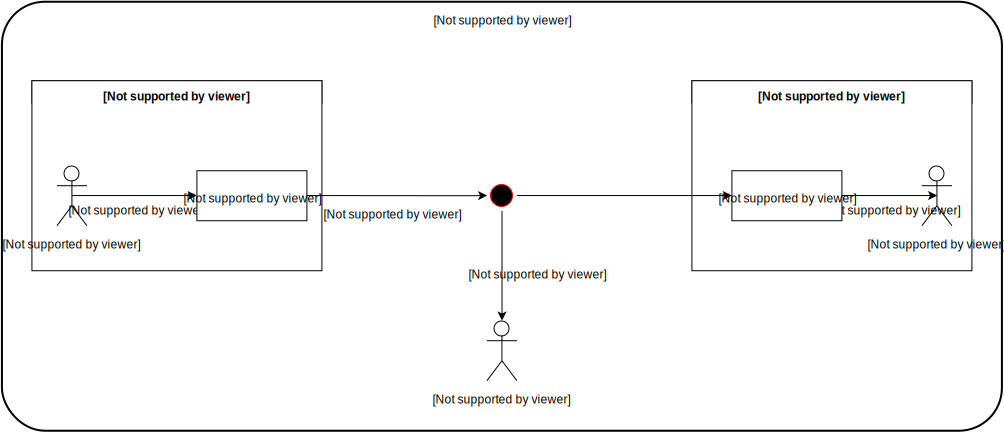
\includegraphics[width=0.8\textwidth]{figures/EAV.png}
        \caption{Eavesdropping (EAV)}
    \end{figure}
\end{frame}


\subsection{Known-plaintext attack (KPA)}
\begin{frame}{Known-plaintext attack (KPA)}
    
    \begin{figure}[h]
        \centering
        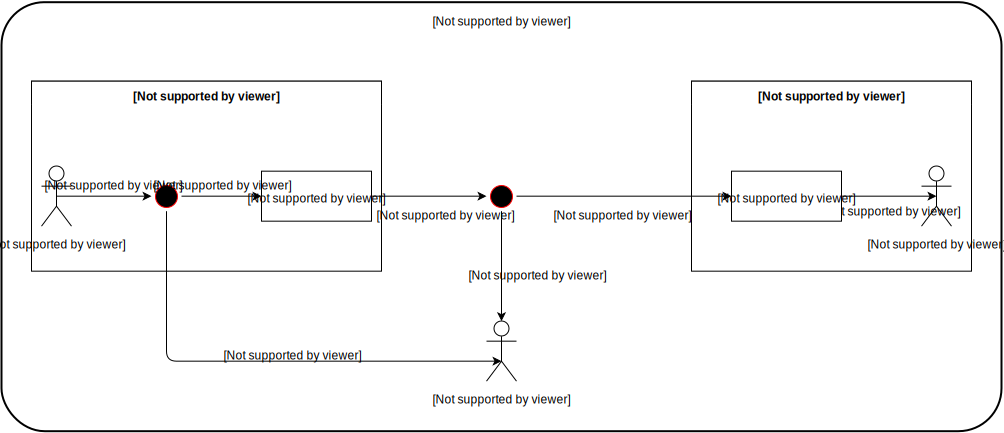
\includegraphics[width=0.8\textwidth]{figures/KPA.png}
        \caption{Known-plaintext attack (KPA)}
    \end{figure}
\end{frame}


\subsection{Chosen-plaintext attack (CPA)}
\begin{frame}{Chosen-plaintext attack (CPA)}
    
    \begin{figure}[h]
        \centering
        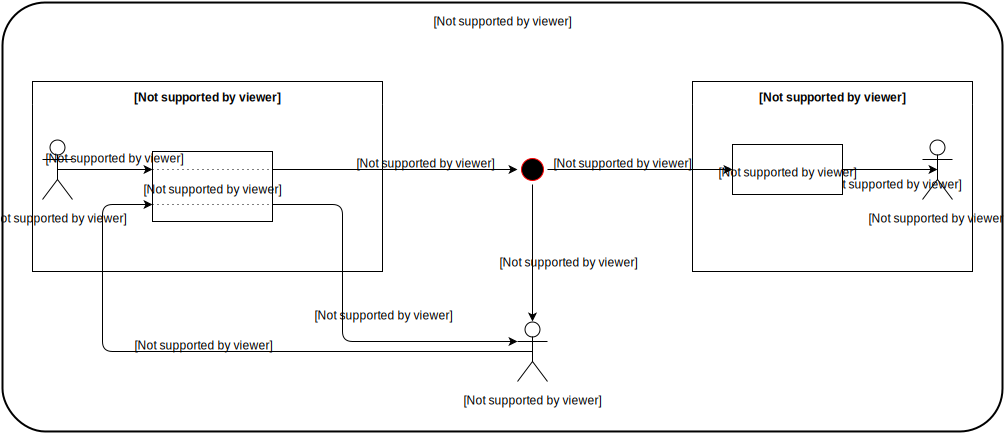
\includegraphics[width=0.8\textwidth]{figures/CPA.png}
        \caption{Chosen-plaintext attack (CPA)}
    \end{figure}
\end{frame}


\subsection{Chosen-ciphertext attack (CCA)}
\begin{frame}{Chosen-ciphertext attack (CCA)}
    
    \begin{figure}[h]
        \centering
        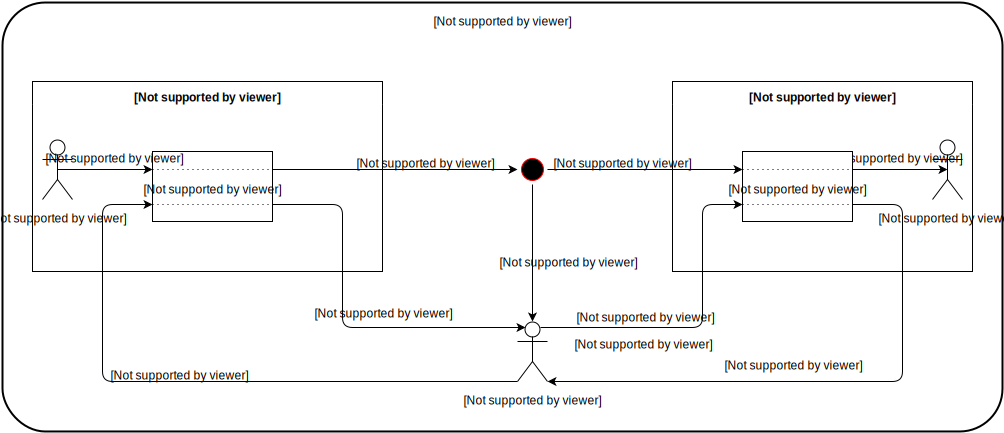
\includegraphics[width=0.8\textwidth]{figures/CCA.png}
        \caption{Chosen-ciphertext attack (CCA)}
    \end{figure}
    
\end{frame}

\begin{frame}{Chosen-ciphertext attack (CCA)}
    \begin{block}{The CCA indistinguishability experiment $ PrivK_{A,\Pi}^{cca}(n) $}
        $\Pi = (Gen, Enc, Dec)$ is any private-key encryption scheme\\
        $A$ is the adversary\\
        $n$ is the security paramter\\
        \begin{enumerate}
            \item $ k \overset{\$}{\leftarrow} Gen(1^n) $
            \item $ m_{0}, m_{1} \leftarrow A^{Enc_{k}(.), Dec_{k}(.)}(ask, 1^{n}) $
            \item $ b \overset{\$}{\leftarrow} \{0, 1\} $
            \item $ c \leftarrow Enc_{k}(m_{b}) $
            \item $ b' \leftarrow A^{Enc_{k}(.), Dec_{k}(.)}(guess, c) $
            \item $ if\ b == b'\ output\ 1 $ \\
            $ else\ output\ 0 $
        \end{enumerate}
    \end{block}
\end{frame}

\section{Signature schemes}
\begin{frame}
    \centering
    \huge{Signature schemes}
\end{frame}

\subsection{Adaptive-chosen-message attack (ACMA)}

\begin{frame}{Adaptive-chosen-message attack (ACMA)}
    \begin{figure}[h]
        \centering
        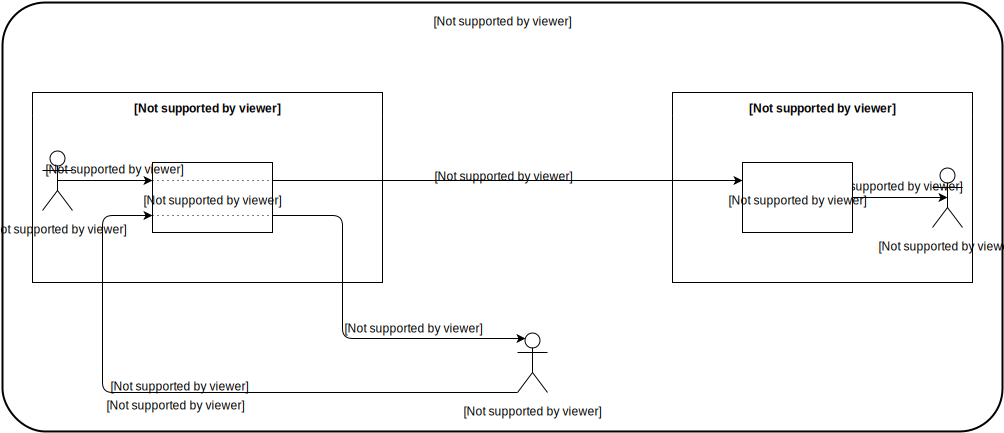
\includegraphics[width=0.5\textwidth]{figures/ACMA.png}
        \caption{Adaptive-chosen-message attack (ACMA)}
    \end{figure}
\end{frame}


\section*{Questions}

\begin{frame}{Questions}
    \huge{Any annotations or questions?}
\end{frame}
\end{document}
